\noindent Here we complete our discussion of SSB in the context of gauge theories (e.g., the Higgs mechanism), and give a broad overview of open questions and where to go next. \\

\noindent Recall from the previous lecture we began working with a local gauge theory of bosons with a tuple of independent scalar fields $\begin{pmatrix} \phi_1 \\ \vdots \\ \phi_d \end{pmatrix}$. Each field transforms according to the local gauge symmetry

\begin{equation}
\phi_j \rightarrow (1 + i \alpha^a t^a)_{jk} \phi_k
\end{equation}

\noindent Where the $t^a$ is a purely imaginary representation. \\

\noindent Next, we added a potential to the Lagrangian density that is minimized by some configuration $\phi_0 = \text{arg}_{\phi} \text{min} (V(\phi))$. If this minimal configuration is not equal to zero $\phi_0 \ne 0$, then we can spontaneously generate mass. For example, we choose, via gauge invariance, an eigenvector with just one nonzero value to be the minimal configuration

\begin{equation}
\phi_0 = \begin{pmatrix} 0 \\ \vdots \\ \nu \end{pmatrix} \equiv \begin{pmatrix} \underline{0} \\ \nu \end{pmatrix}.
\end{equation}

\noindent To understand how the gauge bosons acquire mass, consider the kinetic energy term built with the covariant derivative mod squared $|D_\mu \phi |^2$, since the representation is purely imaginary, which is a long, complicated expression. Expand the fields in this expression around the minimal configuration by writing $\phi = \phi_0 + \phi_1$. This yields another long, complicated expression, but let's focus on the ``mass term'', which allows the spontaneous generation of mass in gauge theory,

\begin{equation}
|D_\mu \phi|^2 = \dots + \frac{1}{2} g^2 m_{ab}^2 A_\mu^a A^{b \mu}
\end{equation}

\noindent Where the mass matrix $m_{ab}^2$ is equal to

\begin{equation}
m_{ab}^2 = \begin{pmatrix} \underline{0} & \nu \end{pmatrix} \tau^a \tau^b \begin{pmatrix} \underline{0} \\ \nu \end{pmatrix}
\end{equation}

\noindent And can be positive semidefinite or negative semidefinite due to the metric. Consider the form of the gauge boson fields in this mass term

\begin{equation}
A_\mu^a A^{b \mu} = A^a_0 A^b_0 - A_1^a A_1^b - A_2^a A_2^b - A_3^a A_3^b   .
\end{equation}

\noindent The only non-negative term is the zeroth, timelike, longitudinal element, and will cause the entire term to not look like a mass term. The three spatial degrees of freedom in this expression, if $m^2_{ab}$ is positive semidefinite, will lead to a mass term in the Lagrangian density $\mathcal{L}$, since mass terms have a minus sign in $\mathcal{L}$. \\

\noindent The longitudinal term does not look right and can be cancelled off since, for the photon, momentum only has transverse components: no longitudinal components. Consider the vacuum polarization diagram like we sketched in the previous lecture for the Abelian Higgs model.

\begin{figure}[H]
	\centering
	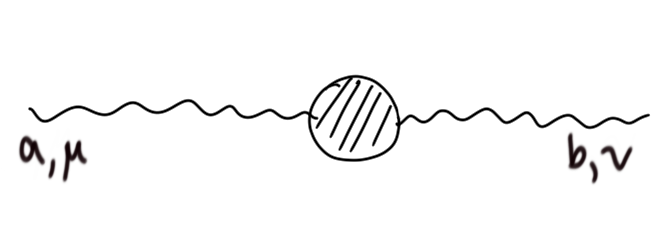
\includegraphics[width=2in]{images/gauge_boson_poles.png}
\end{figure} 

\noindent The contributing diagram in the propagation of a gauge boson, which cancels off the longitudinal term in the perturbation expansion, is a second order term involving the exchange of a fermion.

\begin{figure}[H]
	\centering
	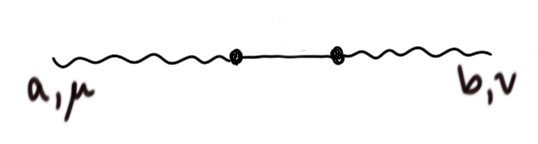
\includegraphics[width=2in]{images/gauge_boson_cancel.png}
\end{figure} 

\noindent This diagram contributes the \textit{purely transverse term}, with longitudinal contributions cancelled off,

\begin{equation}
i m_{ab}^2 \left( \eta^{\mu\nu} - \frac{k^\mu k^\nu}{k^2} \right).
\end{equation}

\noindent In the previous lecture, we worked out the fundamental representation of $SU(2)$ for the gauge theory. In this representation, work out the kinetic energy $\sim |D_\mu \phi|^2$ and find that

\begin{equation}
m_{ab}^2 \propto \mathbb{I}_{ab}.
\end{equation}

\noindent With the mass term proportional to the identity, this means that all three gauge bosons in this gauge theory have the same mass. Now, how do we build a gauge theory that gives mass to some gauge bosons but not others? \\

\subsection*{Glashow-Weinberg-Salam (GWS) Theory of Weak Interactions}

\noindent The GWS theory of weak interactions is a theory to describe gauge boson and electromagnetic field (photon) interactions in one theory. The local gauge group which this theory is invariant under is $SU(2) \times U(1)$. The gauge group symmetry transformations act on gauge boson fields as

\begin{equation}
\phi \rightarrow e^{i \alpha^a \tau^a} e^{i \frac{\beta}{2}} \phi
\end{equation}

\noindent Where $\tau^a = \frac{\sigma^a}{2}$ are the Pauli spin matrices from the $SU(2)$ (gauge boson) part of the group, and $\beta$ is a scalar from the $U(1)$ (photon) part of the group. Think of the action of $U(1)$ as giving charge to the field $\phi$. \\

\noindent Now add the potential $V(\phi)$ to the Lagrangian density and minimize the potential such that

\begin{equation}
\phi = \phi_0 + \phi_1 \, \text{ , where } \phi_0 = \frac{1}{\sqrt{2}} \begin{pmatrix} 0 \\ \nu . \end{pmatrix}
\end{equation}

\noindent Expand the covariant derivative around the minima $\phi_0$, and in the fundamental representation for this gauge group $SU(2) \times U(1)$, we get (\textbf{Exercise})

\begin{equation}
D_\mu \phi = (\partial_\mu - i g A_\mu^a \tau^a - \frac{i}{2} g' B_\mu ) \phi
\end{equation}

\noindent With the connection gauge field $\begin{pmatrix} A_\mu^a \\ B_\mu \end{pmatrix} \sim \begin{pmatrix} SU(2) \\ U(1) \end{pmatrix}$. Putting everything together into a locally gauge invariant Lagrangian density

\begin{equation}
\mathcal{L}_{\text{GWS}} = |D_\mu \phi|^2 - \frac{1}{4}F_{\mu\nu}F^{\mu\nu} + \dots + \text{fermion term} + \dots + V(\phi).
\end{equation}

\noindent The fermion term will be discussed below. \\

\subsubsection*{Mass Generation}

\noindent Due to the potential having a minimum configuration, we can generate mass in this gauge theory to endow gauge bosons with mass. We want to do this, because massive bosons are experimentally observed. Expand the Lagrangian density around the minima $\phi_0$ and acquire a term from the kinetic energy term that looks like (\textbf{Exercise})

\begin{equation}
\text{``mass term''} \equiv \frac{\nu^2}{8} \left( g^2 (A_\mu^1)^2 + g' (A_\mu^2)^2 + (ig A_\mu^3 + g' B_\mu)^2 \right).
\end{equation}

\noindent So, $A_\mu^1$,$ A_\mu^2$, and the combination of fields $A_\mu^3$/$B_\mu$ each act like they have a mass, interpreted as massive gauge bosons: three degrees of freedom from $SU(2)$. The fourth degree of freedom is missing from this mass term, and we, therefore, conclude that it does not have a mass, and we interpet this as the photon: one degree of freedom from $U(1)$. \\

\noindent It is convenient to rename the fields

\begin{align}
W_\mu^\pm &= \frac{1}{\sqrt{2}} \left( A_\mu^1 \mp i A_\mu^2 \right) \\
Z_\mu^0 &= \frac{1}{\sqrt{g^2 + g'^2}} \left( g A_\mu^3 - g' B_\mu \right)
\end{align}

\noindent With masses

\begin{align}
m_W &= \frac{1}{2} g \nu \\
m_Z &= \frac{1}{2} \sqrt{g^2 + g'^2} \nu.
\end{align}

\noindent The fourth field (degree of freedom), with zero mass, we call

\begin{equation}
A_\mu = \frac{1}{\sqrt{g^2 + g'^2}} (g' A_\mu^3 + g B_\mu ).
\end{equation}

\subsubsection*{Coupling to Fermions}

\noindent Gauge bosons couple differently to left-handed and right-handed fermions. Recall that the chirality of fermions arose in the development of gamma $\gamma$ matrices and Weyl spinors and the kinetic energy term decouples into

\begin{equation}
\bar{\psi} (i \slashed{\partial}) \psi = \bar{\psi}_L (i \slashed{\partial}) \psi_L + \bar{\psi}_R (i \slashed{\partial}) \psi_R.
\end{equation}

\noindent Similarly, in the gauge theory

\begin{equation}
\bar{\psi} (i \slashed{D}) \psi = \bar{\psi}_L (i \slashed{D}) \psi_L + \bar{\psi}_R (i \slashed{D}) \psi_R.
\end{equation}

\noindent To recognize this difference in chirality and coupling of gauge bosons to fermions, recall that we have the choice of representation of the gauge group $SU(2)$, and the left- and right-handed fermions can be separated into different representations.

\clearpage

\subsection*{Next Steps}

\noindent There are three ways to go from here:

\begin{enumerate}
\item Practical calculations for experiments, 
\item Physics-focused research,
\item Mathematics-focused research.
\end{enumerate}

\subsubsection*{Physics}

\begin{itemize}
\item Supersymmetry (SUSY)
	\subitem Upgrading symmetries of groups (e.g., Poincar\'e $\rightarrow$ Super Poincar\'e).
\item Quantum gravity via field theory tools (e.g., superstring theory, loop quantum gravity).
	\subitem Superstring theory offers a correct effective theory to explain the high energy physics of black holes.
\item Linear quantum gravity
	\subitem Does not lead to strings.
	\subitem Non-renormalizable theory.
	\subitem Treats the metric $g^{\mu\nu} = \eta^{\mu\nu} + \delta g^{\mu\nu}$ as the degree of freedom.
\item Linear quantum gravity with the Standard Model
	\subitem Only works up to some cutoff $\Lambda$, making an \textit{effective, low energy} theory of gravity. 
	\subitem Best theory we have to date for describing \textit{all} experiments, but we also believe that it is not fundamental, since black holes exist, which conflict with the imposed cutoff, and this theory fails at high energy predictions.
\item AdS/CFT Correspondence
	\subitem Exaplins quantum gravity with field theory alone, no strings.
	\subitem It states that a strongly interacting conformal quantum field theory (CFT) on the boundary of Anti-de Sitter spacetime (AdS) is dual to a quantum gravity theory of Anti-de Sitter spacetime (solutions to Einstein's equations) in its semiclassical limit, which implies that quantum gravity is itself a quantum field theory.
	\subitem We'd prefer to develop this theory in de Sitter spacetime, as that is the spacetime that we find ourselves in (see the work of Strominger).
\item Quantum information theory is becoming helpful to study the kinematics of quantum systems (e.g., photon entanglement).
\end{itemize}

\subsubsection*{Mathematics}

\noindent There are many rigorous formulations of quantum field theory:

\begin{itemize}
\item Axiomatic QFT,
\item Constructive QFT,
\item Functional integration, expansions, and probabilistic approaches,
\item Vertex operator algebras,
\item Chiral \& factorization algebras,
\item Topological QFT (TQFT) \& n-categories.
\end{itemize}

\noindent Why is QFT so difficult to make rigorous? \\

\noindent This is largely in part due to perturbation theory working so darn well, and it is used as the only \textit{standard} tool in QFT at large, but it is wrong, and we know why it is wrong. For example, consider a Gaussian path integral in a $(0+1)$-dimensional QFT with a quartic interaction $Z = \int_{-\infty}^\infty dx \, e^{-x^2 - g x^4}$. As prescribed, we assume that $g$ is small, do perturbation theory, get lots of terms, and end up with a zero radius of convergence! The interaction term does improve convergence, but perturbation theory can't see that. Even after Wick rotation of the path integral $Z = \int \mathcal{D} \phi \, e^{-S}$, which also improves convergence, perturbation theory can't calculate a finitie value for the path integral. Also note that for spacetime dimensions $d>6$, all QFTs are trivial (e.g., Gaussians). \\

\begin{itemize}
\item Axiomatic QFT
	\subitem Wightman: fields are distribution-valued objects (unbounded operators) acting on a Hilbert space.
	\subitem Hang-Kastler: $C^*$-algebras.
	\subitem Osterwalter-Schrader: statistical mechanical foundation (Wick-rotated).
	\subitem Reconstruction theorems: With all $n$-point correlation functions well-behaved, we can reconstruct full Hilbert space and the unitary representations of the Poincar\'e symmetry group.
	\subitem There are problems with local gauge theories (current research).
\item Constructive QFT
	\subitem Cluster expansions takes the Wick-rotated, Euclidean path integral and trade off the low energy perturbation series expansion for estimates of large values of the degrees of freedom that suppress bad parts of the series to get finite results.
	\subitem Successful in $(1+1)$- and $(2+1)$-dimensional spacetime, as well as local gauge theory, but it is very intricate and has become very difficult to communicate and check results.
\item Algebraic QFT
	\subitem Start with some axioms and abstract what the observables should be from there.
	\subitem Quantifies locality in the algebra, leading to observable ($C^*$) algebras.
	\subitem There is difficulty in finding the states ($n$-point function) to match the $C^*$ algebras.
\item Functional integration, expansions, and probabilistic approaches
	\subitem Nelson's axioms are stronger than the Osterwalter-Schrader axioms.
\item Vertex operator algebras
	\subitem Very successful with conformal field theories (CFTs), but is stuck in $(1+1)$ dimensions.
\item TQFT \& n-categories
	\subitem Exactly solvable, strongly interacting theories built on n-categories.
\item Chiral \& factorization algebras
	\subitem See the work of Costello on perturbation expansions.
\item Mathematical theory of effective QFT
	\subitem Follows the work of Wilson.
\end{itemize}

